% !TEX root = ../main.tex
% !TEX program = XeLaTeX
% !TEX encoding = UTF-8 Unicode

\date{2018년 3월 28일}

\begin{frontmatter}
\title{축치어}
\author{양재영}
\address{서울대학교}
\begin{abstract}
Dunn, Michael. (1999). A Grammar of Chukchi. PhD dissertation, Australian National University, 119--174.
\end{abstract}
\end{frontmatter}

%%%%%

\section*{발제 범위 분배}
\begin{table}[h]
\begin{center}
\def\arraystretch{1.5}
\begin{tabular}{>{\sffamily}ccccl}
\hline
	&\itshape 발제자	&\itshape 발제 범위		
	&\itshape 페이지	&\itshape 내용\\
\hline
1	&김민규	&Ch. 1--3	&pp. 1--60		&서론, 방언, 음운론 \& 형태음운론\\
2	&양재영	&Ch. 4--6	&pp. 61--118	&품사, 문장, 명사류 굴절\\
3	&양재영	&Ch. 7--9	&pp. 119--174	&대명사, 명사류 파생, 복합 명사류\\
4	&		&Ch. 10--11	&pp. 175--220	&동사 굴절, 결합가\\
5	&		&Ch. 12--13	&pp. 221--252	&동사 포합, 비정형 동사파생 형태\\
6	&		&Ch. 14--15	&pp. 253--290	&동사 파생, 장소적 관계\\
7	&		&Ch. 16--17	&pp. 291--324	&형용사 \& 수사, 계사 \& 보조사\\
8	&		&Ch. 18--19	&pp. 325--360	&부정문, 화용론\\
\hline
\end{tabular}
\end{center}
\label{default}
\end{table}

%%%%%
들어가기 전에...
\begin{itemize}
	\item 축치어는 주제 중심 능격 체계 교착어입니다.
	\item 축치어의 품사에는 명사류(명사, 대명사, 분사), 형용사, 수사, 굴절 동사(inflecting verb), 동사 어기(verb base; 조동사와 함께 분석적 동사 형성), 부동사(converb), 부사/불변화사(소사; particle)가 있습니다.
	\item 축치어 명사류는 단/복수(+개별), 인칭, 격에 따라 상당히 규칙적으로 곡용하며, 그 패턴은 생물성에 따라 보통명사와 고등 생물 명사로 나뉩니다.
	\item 축치어의 격에는 절대격, 능격/(도)구격, 등격(equative), 처(소)격, 향격, 탈격, 통격(perlative), 종격(orientative), 내격(inessive), 하격(sublative), 참여격(associative), 공동격(comitative), 결여격(privative) 총 13개가 있습니다.
\end{itemize}

\setcounter{section}{6}
\section{대명사}
\subsection{서론}
축치어는 동사, 명사, 형용사에 붙는 다양한 의존 대명사적 형태소와 네 종류의 독립 대명사로 대명사적 지시 기능을 수행한다. 전자는 이후에 소개할 것이고, 후자는 다음과 같다.
\begin{enumerate}
	\item \textbf{인칭 대명사}에는 1/2/3인칭 단/복수에 따른 여섯 가지 어간이 있으며, 격 표지와 지소/확대 등의 파생을 받는다.
	\item \textbf{부정不定/의문 대명사}에는 유정('누구, 누군가')/무정('무엇, 무언가')의 두 가지 어간이 있다.
	\item \textbf{지시 대명사}는 직시 및 대용 기능을 하며, 그 중 하나는 대용에 특화되어 있다.
	\item \textbf{양화 대명사} 어간으로는 \textbf{əməlˀo} `모두'와 \textbf{qut-} `(-- 중) 하나/일부'가 있다.
\end{enumerate}
뒤의 세 종류는 명사구의 수식어일 때 핵어 명사와 수 일치를 할 수 있으나 명사구에 복수성이 명시적으로 표시되는 경우 종종 생략된다. 절대격 대명사처럼 행동하지만 다른 격은 받지 않는 `논항성' 불변화사로는 양화사 \textbf{cəmqək}, 재귀 부사 \textbf{cinit}, 재귀 대명사 \textbf{cinitkin(e)-} 및 여러 한정 대명사성 부사들이 있다.
\subsection{인칭 대명사}
인칭 대명사의 절대격 어간과 사격 어간은 아래와 같이 다르다.
\begin{figure}[H]
\centerline{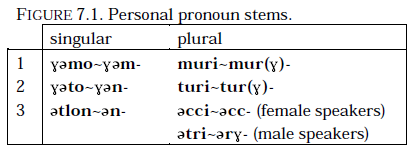
\includegraphics{Chukchi/src/chpp.png}}
\end{figure}
동사에 필수 대명사적 공지시가 발달해 있어, 독립 인칭 대명사는 특수한 담화상의 기능(대조, 접속 명사구의 일부, 인용 발화에서 가상의 화행 참여자 구분)에 쓰인다. 대용어로서나 계사절에서도 잘 나오지 않으나, 동사 공지시가 없는 격 기능의 경우 독립 대명사를 사용할 수밖에 없다. 3인칭 대명사는 대화나 인용에서 강조 소사로도 쓰이는데, 단수형은 의문문, 복수형은 미래에 대한 진술에서 쓰인다.
\begin{figure}[H]
\centerline{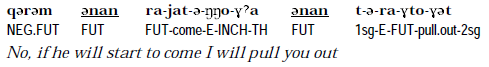
\includegraphics{Chukchi/src/chfu.png}}
\end{figure}
\begin{itemize}
	\item \textbf{대조}적이거나 기대에 반하는 논항을 강조하는 데 사용된다. 
	\item \textbf{접속 명사구}에서 담화 조건과 관계없이 독립 대명사가 쓰인다.
	\item \textbf{인용 발화}에서는 직접 발화보다 독립 대명사가 빈번하게 나타난다.
\end{itemize}
\subsection{부정/의문 대명사}
유정/무정형 모두 절대격과 사격 어간이 다르다.
\begin{figure}[H]
\centerline{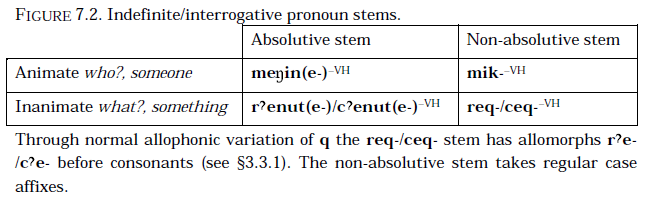
\includegraphics{Chukchi/src/chii.png}}
\end{figure}
부정과 의문 기능은 맥락으로 (특히 억양으로) 구별되며, 많은 언어와 달리 단 하나의 부정 대명사만 존재한다. 부정 대명사의 지시체는 특정한 알려진 것, 특정한 모르는 것, 불특정한 것 모두 가능하며 판정 의문문이나 조건문에서도 사용된다. 부정否定시에는 결여격을 쓰기도 하나 (이 경우 존재 부정) 부정문에 그대로 쓰이기도 한다. `비교 기준'과 `자유 선택' 기능은 정보가 없다. 접두사 \textbf{im-}이 붙으면 `모든 것'이라는 의미의 대명사로 파생되며 이 경우 의문적 해석은 불가능하다. 아래와 같이 의문 대명사의 포합이 가능하다.
\begin{figure}[H]
\centerline{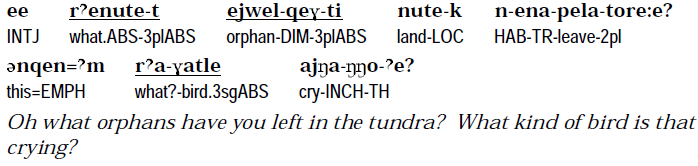
\includegraphics{Chukchi/src/chqi.png}}
\end{figure}
\subsection{지시 대명사}
대부분은 지시 부사/소사와 동일한 어간에서 형성되며 화자로부터의 거리를 구분한다.
\begin{figure}[H]
\centerline{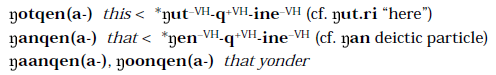
\includegraphics{Chukchi/src/chde.png}}
\end{figure}
\begin{figure}[H]
\centerline{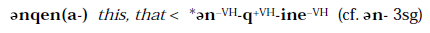
\includegraphics{Chukchi/src/chan.png}}
\end{figure}
대용 특화 \textbf{ənqən(a-)}를 포함해 모든 지시 대명사는 이전에 언급된 대상의 대용 기능도 한다. \textbf{ənqən(a-)}은 종종 지시 소사 \textbf{waj / raj/caj} 뒤에 나오며, 하나의 단위로서 주로 새로운 대상을 끌어들일 때 사용한다. \textbf{ŋanqen / ŋaanqen/ŋoonqen}의 3인칭 단수 절대격은 방향적 의미의 지시 부사로 기능한다. \textbf{ŋaanqen/ŋoonqen}의 첫 모음의 길이를 늘림으로써 거리를 강조하기도 한다.
\subsection{양화 대명사}
사격의 경우 고등 생물 명사 곡용을 따르며, 특히 \textbf{əməlˀo}는 복수형처럼 곡용하지만 독립된 절대격 명사구로 나타날 때에는 동사에 단수(영표지) 일치를 하기도 한다. 또한 절대격 명사구 내에서 단/복수 명사류 핵어와 함께 나올 수 있다. \textbf{qut-}는 하나, 다른 하나, 나머지 하나를 의미하는 불규칙 단수형 \textbf{qol}과 일부, 나머지를 의미하는 규칙 복수형이 있다. 후자는 절대격에서는 보통명사, 사격에서는 고등 생물 명사처럼 곡용한다. 명사구 내의 수식어인 경우 핵어의 수에 일치한다. 파생 접미사가 붙거나 포합될 때 이형태 \textbf{qulle-}가 쓰인다.
\begin{figure}[H]
\centerline{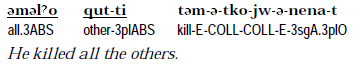
\includegraphics{Chukchi/src/chqu.png}}
\end{figure}
\subsection{논항성 부사}
의미적으로 대명사와 겹치나 격에 따른 형태가 없는 부사들로, \textbf{cəmqək} `다른 이들', \textbf{cinit} `자신'과 \textbf{amɣəmnan} `혼자, 내 스스로', \textbf{ammorɣənan} `혼자, 우리 스스로' 등 인칭이 표시된 제한적 형태가 속한다. 명사구 내에서 수식어로 기능할 수 있기에 부사로 분류한다. 
\subsubsection{양화 부사 cəmqək}
절대격 양화 대명사처럼 행동하지만 형태적 변화가 없고 문법 범주 표시도 없다. 보통은 인간을 지시하나 비인간이나 무정물도 지시할 수 있다.
\subsubsection{재귀 부사와 재귀 관계 대명사}
수식 대상으로 명시적 명사류 논항이 없어도 되며, 동작주성(S\textsubscript{A}/A)을 띠는 논항에만 나타난다. 축치어에는 형태론적 재귀화 방법이 없다. 관계 접미사로 파생된 \textbf{cinitkin} `그 자신'은 대명사로 지시 대상의 통사적 제약이 없으며, `친척, 친족'이라는 의미의 명사로도 쓰인다.
\subsubsection{한정 대명사성 부사}
인칭-수 표시가 가능한 `혼자'라는 의미의 부사들이 있다. 3인칭 단수는 모든 성-수 조합을 대신할 수 있다.
\begin{figure}[H]
\centerline{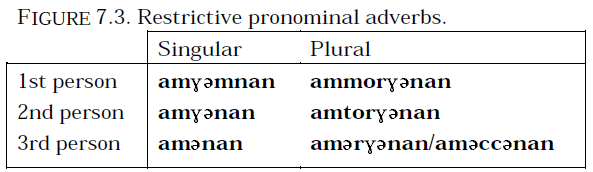
\includegraphics{Chukchi/src/chad.png}}
\end{figure}

\section{명사류 파생}
\subsection{서론}
\omission
\subsection{분사}
긍정 극성에는 능동 분사 접미사 \textbf{-lˀ}와 수동 분사 접미사 \textbf{-jo}(복수형 \textbf{-jot-te})가 있다. 전자는 동사 어간에 \textbf{e$\rangle\langle$kə\textsuperscript{-VH}}나 \textbf{luŋ-}이 붙어 부정되면 동사 어간의 타동성에 따라 능동과 수동 분사를 모두 만들 수 있으며, 다른 품사의 어간에서도 명사를 파생시킨다. 후자는 귀결적인 의미를 갖는다는 점에서 전자와 구별된다. (부정 수동 분사는 과거에 사건이 발생한 적 없으므로 비귀결적이다.) 분사는 절의 논항, 명사구의 핵어 및 수식어로 기능한다. 간혹 수동 분사의 기저 A(동작주)가 도구격으로 나타나기도 하며, 더 드물게는 절대격의 소유 파생 명사로 나타난다. 수동 분사는 절대격 외의 격으로는 잘 나타나지 않으며, 접미사 -jo는 \textbf{-lqəl} 등 특정한 파생 접사가 붙을 때는 필수이다. \textbf{e$\rangle\langle$kə-lˀ-} 조합의 부정 분사는 \textbf{-in(e-)} 어미를 갖고, \textbf{luŋ-} 접두사로 만든 부정 분사는 III부류(\textbf{-n} 어미)에 속한다. 타동사에서 능동 분사를 만들려면 자동사화(역수동태화)가 필요하며, 이는 \textbf{ine-}나 \textbf{-tku} 혹은 목적어 포합으로 가능하다.
\subsection{분사가 아닌 -lˀ-/-cˀ- 파생}
\begin{itemize}
	\item \textbf{공간적 용어}(부사 포함)에 \textbf{-lˀ}이 붙으면 그 장소에서 유래한 사람이나 사물을 의미한다. 예컨대 \textbf{emnuŋ} `툰드라'에서 \textbf{emnuŋ-ə-lˀ-ə-t} `툰드라 사람'이 파생된다. (이는 관계어 \textbf{emnuŋ-kine-t} `툰드라에서 온 (것)'과 대비된다.)
	\item \textbf{물리적 실체}를 나타내는 단어에서 그 존재를 소유하는 사람이나 사물을 파생시킨다.
	\item \textbf{속성}을 나타내는 단어(주로 형용사, 추상명사)에서 그 속성을 가진 존재를 파생시킨다.
\end{itemize}
\textbf{-cˀ-}는 보다 어휘화된 단어를 만든다. 예컨대 \textbf{weriw-ə-lˀ-ə-n} `시다, 신 것'과 \textbf{weriw-ə-cˀ-ə-n} `월귤나무 열매'.
\subsection{행위 명사 파생 (-ɣərɣ-\textsuperscript{+VH})}
접미사 \textbf{-ɣərɣ-\textsuperscript{+VH}}는 동사(때로 형용사나 명사)에서 `행위 명사'를 파생시키며, 분사와 달리 타동성에 영향을 받지 않는다. 예컨대 \textbf{wˀi-} `죽다'에서 \textbf{wˀe-tko-ɣərɣ-ə-n} `죽음, 역병'이, \textbf{ˀeqe-} `나쁜'과 \textbf{liŋ-} `심장'의 포합 명사에서 \textbf{ˀaqaleŋɣərɣən} `두려움'이 파생된다.
\subsection{명사화 파생}
\begin{itemize}
	\item \textbf{처소 명사화} 접미사 \textbf{-n\textsuperscript{+VH}/-nwə-}는 동작이나 상태를 의미하는 동사에서 그 발생지를 파생시킨다.
	\item \textbf{'시대' 명사화} 접미사 \textbf{-ja}는 소수의 동사/형용사 파생 명사에 붙어 그 어간으로 특징지어지는 시기나 시대를 파생시킨다. 예컨대 \textbf{wˀe-tko-ja-n} `사망의 시기; 역병'. 
	\item \textbf{도구 명사화} 접미사 \textbf{-ineŋ(e-)}는 자동사(화된) 어간에서 도구나 장비를 파생시킨다. 예컨대 \textbf{wˀaj-ə-cwe-tko-naŋ} grass-E-cut-ITER-TOOL.3sgABS `낫'.
	\item \textbf{'용기' 명사화} 접미사 \textbf{-jolɣ-}는 동사나 명사에서 `담고 았는 것'을 의미하는 명사류를 파생시킨다. 예컨대 \textbf{wetɣaw-jolɣ-a-n} speak-CONTAIN-E-3sgABS `라디오'.
\end{itemize}
\subsection{인명}
고등 생물 명사로만 곡용하는 규칙적 명사로, 많은 수는 파생 명사이다. 명사화 접미사 \textbf{-ŋewət}과 \textbf{-wji}(남성)는 인명에만 쓰인다. 여성 인명은 종종 (모든 동물의 암컷을 파생시키는) \textbf{ŋew-}, (\textbf{ənpaŋew} `노파'를 파생시키는) \textbf{-ŋew}, \textbf{-ŋewət}으로 형성된다.
\subsection{소유와 관계}
\begin{itemize}
	\item \textbf{소유 접미사 -in(e)-}는 소유주 명사에 붙어 소유 구문을 만든다.
	\item \textbf{관계 접미사 -kin(e)-}는 소유 접미사와 동일한 행동을 보이나, 근원, 기원, 의도의 의미를 가진다.
	\item 명사화 접미사 \textbf{-lˀ}은 분사 접미사와 동일한 형태로, 명사나 형용사에 붙어 해당 대상/성질의 소유주를 파생시킨다.
	\item 소유주는 피소유물에 접두되어 포합된 소유주 명사류를 만들 수 있다.
	\item 이에 더해 접두사 \textbf{ɣe-}와 대명사적 접미사로 이루어진 피소유 술부 표지가 있다.
\end{itemize}
\subsubsection{소유 접미사 -in(e)-}
격이 아니며, 파생 접미사 뒤에, 격 접미사 앞에 온다. 회귀적인 소유는 드물다. 대명사의 소유 형태는 다음과 같다.
\begin{figure}[H]
\centerline{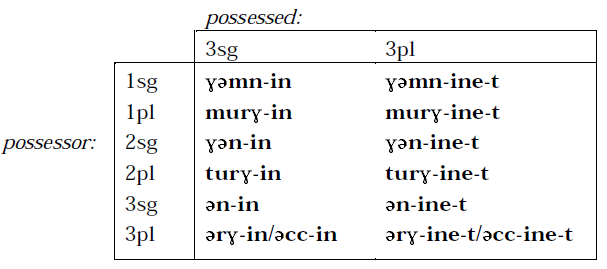
\includegraphics{Chukchi/src/chpo.png}}
\end{figure}
소유되는 존재가 3인칭이 아니면 인칭-수 접미사가 추가된다.
\begin{figure}[H]
\centerline{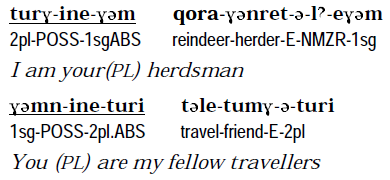
\includegraphics{Chukchi/src/chn3.png}}
\end{figure}
소유주의 복수성은 앞에 \textbf{-rɣ-}를 추가하여 표시한다. `여격'형 의미를 가지는 예시들이 나타난다.
\begin{figure}[H]
\centerline{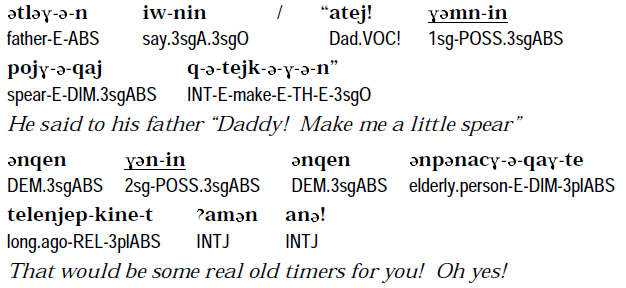
\includegraphics{Chukchi/src/chda.png}}
\end{figure}
\subsubsection{관계 접미사 -kin(e)-}
동격 명사구에 나타나며, 핵어가 기원한 장소/시간이나 의도를 나타낸다. 복수 표시는 소유형과 동일하고, 보통 복수인 핵어가 생략되었을 때 나타난다. 대명사의 관계형은 (소유형에는 붙지 않지만 유표격 형태에는 붙는) \textbf{-ke}를 사이에 넣어 만드나, 핵어가 SAP(핵심 논항)인 경우 대신 \textbf{-ine}가 붙는다.
\begin{figure}[H]
\centerline{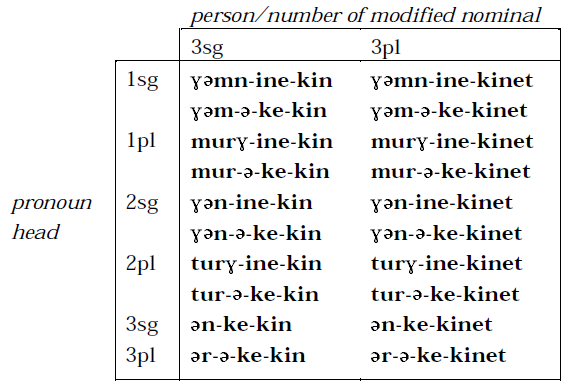
\includegraphics{Chukchi/src/chre.png}}
\end{figure}
\subsection{공간적 파생}
축치어 명사류의 공간 관계는 격, 파생, 부사/후치사의 세 가지 방식으로 표현된다. 그중 파생 접미사에는 다음의 네 가지가 있다.
\begin{figure}[H]
\centerline{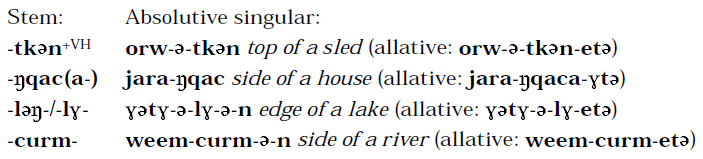
\includegraphics{Chukchi/src/chsp.png}}
\end{figure}
뒤의 둘은 절대격 단수를 \textbf{-n}으로 표시되며, 공간적 파생은 종종 처격이나 향격, 탈격을 받는다. 
\subsection{화자 평가}
지소 접미사 하나와 확대 접미사 둘이 있으며, 형용사 등 다른 품사에도 붙는다.
\subsubsection{지소사}
작음이나 애정을 표현하는 지소 접미사 \textbf{-qej\textsuperscript{-VH}}가 있다.
\subsubsection{확대사}
큼을 나타내는 확대 접미사 \textbf{-jŋ}과 \textbf{-cɣ-}(VC 뒤에서 \textbf{-cəŋ-})이 있다.
\subsection{양적 파생}
명사의 집합 접미사 셋과 다른 품사에도 붙는 여러 양적 접두사들이 있다.
\subsubsection{집합 접미사}
형용사 어간 \textbf{mk} `많은'과 동근인 \textbf{-mk-}가 가장 흔하며, 반복상/역수동태-반복상 접미사와 동형인 \textbf{-tku}와 어떻게 다른지는 확실치 않다. \textbf{-ɣiniw}는 인간 집단을 파생시킨다.
\subsubsection{강의强意 접두사}
강의 접두사 \textbf{lɣi-}와 \textbf{teŋ-\textsuperscript{-VH}}은 대부분의 품사에 붙으나 대명사나 파생된 명사에 가장 흔하게 나타난다.
\begin{figure}[H]
\centerline{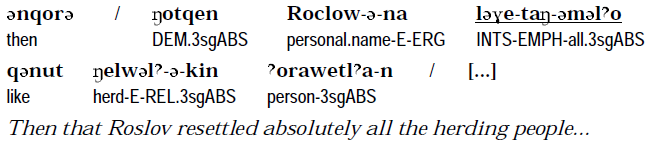
\includegraphics{Chukchi/src/chin2.png}}
\end{figure}
\subsubsection{대략적 및 한정적 접미사}
한정적 접두사 \textbf{em-\textsuperscript{-VH}} `-만'은 명사와 부사, 대략적 접미사 \textbf{mel-\textsuperscript{-VH}} `아마'는 명사와 형용사, \textbf{mec-\textsuperscript{-VH}}는 명사, 동사, 부사에 흔하게 붙는다. \textbf{em-}은 도구격 인칭대명사에 붙어 `스스로'를 뜻하는 부사가 된다.
\subsection{기타 어휘적 접사}
접두사 \textbf{lɣi-}는 축치의 자기 민족명인 \textbf{ləɣ-ˀorawetlˀa-n} (AUTH-person-3sgABS)에서처럼 `진정한, 평소의, 전통적인 종류의 대상'을 의미한다. 접미사 \textbf{-tˀul}은 `--의 조각'을 의미하며 동물 유래 식품의 이름에 흔하다.

\section{복합 명사류}
\subsection{서론}
축치어 명사구는 절대격에서만 나타날 수 있다는 점에서 제한적이며(능격 명사구는 예외), 다른 격에서는 항상 수식어가 핵어에 포합되어 하나의 단어를 이룬다.
\subsection{명사구}
명사구를 이루는 핵어와 수식어는 모두 같은 대상을 지시하며, 수식어는 앞뒤로 올 수 있고 그 종류에는 
\begin{itemize}
	\item \textbf{독립 대명사} 중 인칭 대명사를 제외한 나머지,
	\item \textbf{명사}(분사, 소유형/관계형, 사격 명사 포함),
	\item \textbf{형용사},
	\item \textbf{수사}가 있다.
\end{itemize}
명사구 내 수식어는 대명사 및 소유형을 제외하면 (이들도 핵어가 생략된 경우에는) 수 일치를 보일 수 있다. 선호되는 선형적 순서는 없으나 명사구 내의 성분들은 문법 요소일수록 핵어에서 멀고, 어휘 요소일수록 가깝다. 이를 도식화하면 다음과 같다.
\begin{figure}[H]
\centerline{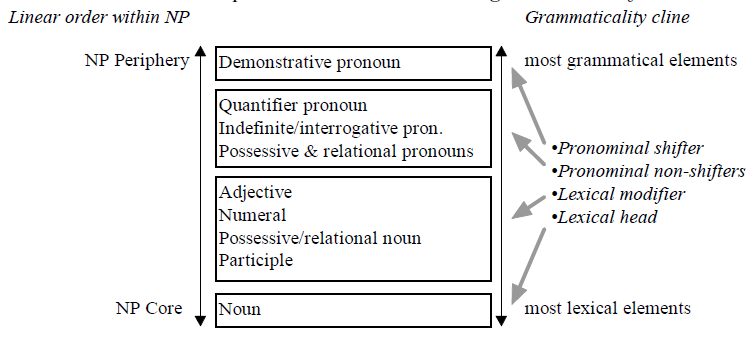
\includegraphics{Chukchi/src/chnp.png}}
\end{figure}
\subsubsection{독립 대명사 수식어}
지시 대명사, 양화 대명사, 부정/의문 대명사가 가능하다. 독립 인칭 대명사는 명사구 수식어로 기능하지 않으며, 명사의 인칭 표시는 대명사적 접미사로 표시된다.
\subsubsection{분사 및 소유/관계 수식어}
\omission
\subsubsection{사격 명사 수식어}
공동격과 참여격은 수식어 기능을 하지만 그 수식 범위는 불분명하다. 명시적 명사류 주어가 없는 문장에 자주 나오며, 명시적 명사가 있으면 참여격이 훨씬 흔하게 쓰인다.
\subsubsection{수식어 형용사}
절대격이 아닌 명사류를 수식할 때는 항상 포합된다. 실질화(substantivization)되는 경우는 격과 수식을 받지 않으므로 핵어 생략으로 보는 것이 타당하다.
\subsubsection{수식어 수사}
\begin{figure}[H]
\centerline{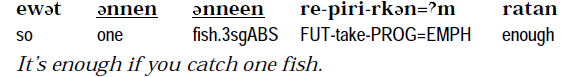
\includegraphics{Chukchi/src/chnu.png}}
\end{figure}
\begin{figure}[H]
\centerline{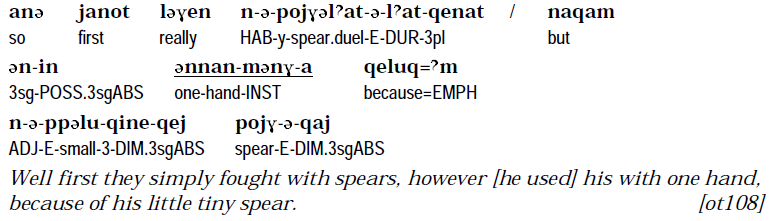
\includegraphics{Chukchi/src/chno.png}}
\end{figure}
\subsection{능격 명사류 구}
매우 드물고, 문법적으로 가능한 구라면 상당히 유표적일 것이다.
\begin{figure}[H]
\centerline{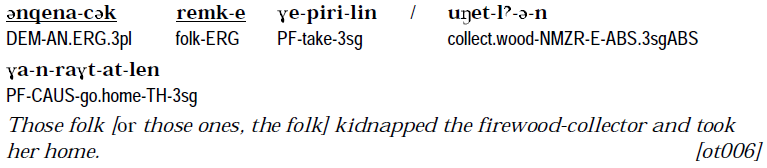
\includegraphics{Chukchi/src/cher.png}}
\end{figure}
\subsection{명사류 포합}
절대격 이외에서 복잡한 의미의 명사류를 나타내려면, 절대격 구를 도입한 후 그것을 다른 단어로 지시하든지, 통사적 포합을 통해 하나의 단어로 만들어야 한다. 물론 절대격 명사류도 화용적 중요도에 따라 수식어 포합이 가능하다. 셋 이상의 어휘적 어간을 포합하는 것은 특이하고 우습게 여겨지며, 일례로 \textbf{kawrajelɣəmelɣətanŋən} `혀 꼬부라진 성냥 이방인'이라는 단어가 유행한 적 있다.
\subsubsection{형용사, 대명사, 수사 수식어}
유형론적으로 이상하지만, 축치어는 한정 형용사뿐 아니라 지시사나 대명사 소유주 등을 통사적으로 포합할 수 있다. 
\subsubsection{명사 수식어}
보통 재료나 출신지를 나타낸다. 아래는 고유명사(지명)이 포합된 예이다.
\begin{figure}[H]
\centerline{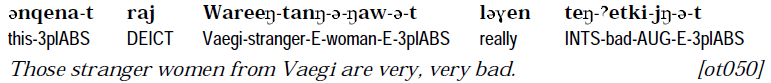
\includegraphics{Chukchi/src/chpn.png}}
\end{figure}
\subsubsection{동사 및 부사 수식어}
동사 수식어는 행위나 상태를 나타낸다. 
\subsection{접속}
참여적 접속 구문과 접속 소사를 이용하는 두 가지 방식이 있다. 전자는 한쪽에 다른 한쪽이 포함되는 경우, 후자는 서로 위계가 동등한 경우 사용한다.
\subsubsection{참여적 접속}
집합적 의미의 복수 핵어(상위어; 주로 인칭대명사나 명사)와 그 집합에 속하는 개체(들)을 가리키는 명사류로 구성되는 구문이다. (참여격이 부분 전체 관계인 명사에 쓰이는 것을 참조하라.) 두 명사류가 모두 절대격이지만 동사 일치는 상위어에 맞춘다. 
\subsubsection{접속 소사}
명사류와 함께 나오는 두 가지 전형적인 접속 소사는 \textbf{ənkˀam}과 \textbf{əmə}로, 동사나 절을 접속시키거나 억양구(문장)를 시작하는 기능도 한다. 후자는 셋 이상의 명사류를 나열할 때 보통 마지막 요소 앞에 쓰인다. \textbf{cama}는 원래 절을 접속시키지만 때로 명사구에도 쓰인다. 아래 예문의 두 접속 요소가 동사 어간에서 파생된 명사라는 점은 우연이 아닐 것이다.
\begin{figure}[H]
\centerline{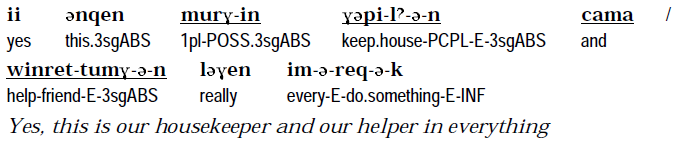
\includegraphics{Chukchi/src/chco.png}}
\end{figure}